\documentclass[border=6pt]{standalone}

\usepackage{tikz}
\usepackage{pgfplots}
\pgfplotsset{compat=1.18}

\begin{document}
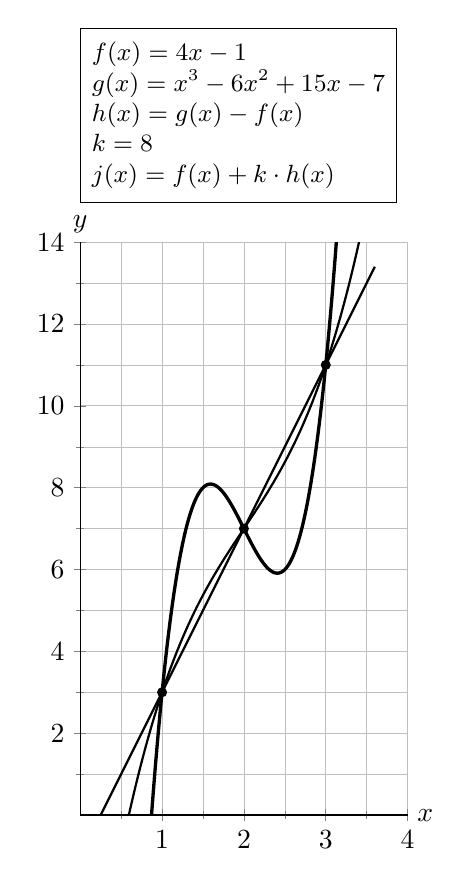
\begin{tikzpicture}
\begin{axis}[
  axis lines=middle,
  axis line style={-},
  unit vector ratio*=2 1 1,
  scale only axis,
  xmin=0, xmax=4,
  ymin=0, ymax=14.0,
  xtick={0,1,2,3,4},
  ytick={0,2,4,6,8,10,12,14},
  grid=both,
  major grid style={line width=0.3pt},
  minor grid style={line width=0.2pt},
  minor tick num=1,
  xlabel={$x$},
  ylabel={$y$},
  xlabel style={right},
  ylabel style={above},
  clip=true,
]

% f(x)=4x-1
\addplot[domain=0:3.6, samples=200, thick] {4*x - 1};

% g(x)=x^3-6x^2+15x-7
\addplot[domain=0:3.6, samples=400, thick] {x^3 - 6*x^2 + 15*x - 7};

% h(x)=g(x)-f(x)=x^3-6x^2+11x-6 (not plotted, used in j)
% j(x)=f(x)+k*h(x). Choose k=8 (as in the screenshot).
\addplot[domain=0:3.6, samples=600, very thick]
  { (4*x - 1) + 8*(x^3 - 6*x^2 + 11*x - 6) };

% intersection points (1,3), (2,7), (3,11) stay fixed for all k
\addplot[
  only marks,
  mark=*,
  mark size=1.6pt
] coordinates {(1,3) (2,7) (3,11)};

\end{axis}

\node[
  draw,
  fill=white,
  anchor=north west,
  inner sep=4pt,
  font=\small
] at (0,10) {%
  \begin{tabular}{@{}l@{}}
    $f(x)=4x-1$\\
    $g(x)=x^3-6x^2+15x-7$\\
    $h(x)=g(x)-f(x)$\\
    $k=8$\\
    $j(x)=f(x)+k\cdot h(x)$
  \end{tabular}%
};
\end{tikzpicture}
\end{document}
